%%%%%%%%%%%%%%%%%%%%%%%%%%%%%%%%%%%%%%%%%%%%%%%%%%%%%%%%%%%%%%%%%%%%%%%%%%%%%%%
%  Curriculum Vitae -- Bartosz Jan Bednarczyk
%  Compile with XeLaTeX or LuaLaTeX, twice:   xelatex cv && xelatex cv
%  Needs photo.jpg next to this file (or put \showphotofalse below).
%%%%%%%%%%%%%%%%%%%%%%%%%%%%%%%%%%%%%%%%%%%%%%%%%%%%%%%%%%%%%%%%%%%%%%%%%%%%%%%
\documentclass[10pt,a4paper]{article}
%%%%%%%%%%%%%%%%%%%%%%%%%%%%%%%%%%%%%%%%%%%%%%%%%%%%%%%%%%%%%%%%%%%%%%%%%%%%%%%
%  settings.tex  --  style for the academic CV of Bartosz Jan Bednarczyk
%  Compile with XeLaTeX or LuaLaTeX, twice:   xelatex cv && xelatex cv
%%%%%%%%%%%%%%%%%%%%%%%%%%%%%%%%%%%%%%%%%%%%%%%%%%%%%%%%%%%%%%%%%%%%%%%%%%%%%%%

% ---------------------------------------------------------------- identity ---
\newcommand{\FirstName}{Bartosz}
\newcommand{\MiddleName}{Jan}
\newcommand{\LastName}{Bednarczyk}
\newcommand{\MyName}{\FirstName\ \MiddleName\ \LastName}
\newcommand{\EmailA}{bartek@cs.uni.wroc.pl}
\newcommand{\EmailB}{bartosz.bednarczyk@tuwien.ac.at}
\newcommand{\Website}{bartoszjanbednarczyk.github.io}
\newcommand{\ORCID}{0000-0002-8267-7554}
\newcommand{\ScholarURL}{https://scholar.google.com/citations?user=j7plXYcAAAAJ}
\newcommand{\DBLPURL}{https://dblp.org/pers/hd/b/Bednarczyk:Bartosz}
\newif\ifshowphoto \showphototrue        % \showphotofalse removes the photo

% ---------------------------------------------------------------- packages ---
\PassOptionsToPackage{table}{xcolor}
\usepackage[english]{babel}
\usepackage{fontspec}
\usepackage[sfdefault,book,lining]{FiraSans}
\defaultfontfeatures{Ligatures=TeX,Numbers=Lining}
\newfontfamily\FiraLight{FiraSans-Light.otf}[BoldFont=FiraSans-SemiBold.otf]
\newfontfamily\FiraSemi{FiraSans-SemiBold.otf}[ItalicFont=FiraSans-SemiBoldItalic.otf]
\newfontfamily\FiraMedium{FiraSans-Medium.otf}
\newfontfamily\FiraBook{FiraSans-Book.otf}[ItalicFont=FiraSans-BookItalic.otf]
\usepackage{fontawesome5}
\usepackage{academicons}
\usepackage[none]{hyphenat}
\usepackage[a4paper,left=18mm,right=18mm,top=16mm,bottom=18mm,footskip=9mm]{geometry}
\usepackage{xcolor}
\usepackage{graphicx}
\usepackage{tikz}
\usetikzlibrary{calc,positioning,arrows.meta,decorations.pathmorphing}
\usepackage[most]{tcolorbox}
\usepackage{enumitem}
\usepackage{fancyhdr}
\usepackage{lastpage}
\usepackage{etoolbox}
\usepackage{needspace}
\usepackage{microtype}
\usepackage{array}
\usepackage{longtable}
\usepackage[hidelinks]{hyperref}
\usepackage{bookmark}

% ------------------------------------------------------------------ colours ---
\definecolor{ink}{HTML}{163A2C}       % deep forest green: headings, sidebar
\definecolor{inksoft}{HTML}{2E5A47}
\definecolor{accent}{HTML}{23875A}    % jade green: the single accent colour
\definecolor{accentlight}{HTML}{9FDDB5}
\definecolor{tint}{HTML}{EDF6F0}      % very light green: cards
\definecolor{paper}{HTML}{F3F7F4}     % zebra rows
\definecolor{gold}{HTML}{B7862B}      % awards only
\definecolor{muted}{HTML}{68746D}
\definecolor{hair}{HTML}{D4DDD7}
\definecolor{text}{HTML}{212B26}

\hypersetup{pdftitle={Curriculum Vitae -- \MyName},pdfauthor={\MyName},
  colorlinks=true,allcolors=accent}

% -------------------------------------------------------------- typography ---
\setlength\parindent{0pt}
\setlength\parskip{0pt}
\linespread{1.1}
\setlist{nosep}
\frenchspacing
\AtBeginDocument{\color{text}}
\newcommand{\muted}[1]{{\color{muted}#1}}
\newcommand{\sep}{\unskip\nobreak\hspace{0.45em}{\color{muted!45}\textbullet}\hspace{0.45em}\ignorespaces}
\newcommand{\semi}[1]{{\FiraSemi #1}}
\newcommand{\MonthName}{\ifcase\month\or January\or February\or March\or April\or May\or June\or
  July\or August\or September\or October\or November\or December\fi}

% --------------------------------------------------------- footer / header ---
\pagestyle{fancy}
\fancyhf{}
\renewcommand{\headrulewidth}{0pt}
\renewcommand{\footrulewidth}{0pt}
\fancyfoot[L]{\footnotesize\color{muted}{\FiraSemi\color{ink}\MyName}\sep Curriculum Vitae\sep Last updated: \MonthName~\the\year}
\fancyfoot[R]{\footnotesize\color{muted}{\FiraSemi\color{accent}\thepage}\,/\,\pageref*{LastPage}}
\fancypagestyle{cover}{\fancyhf{}%
  \fancyfoot[R]{\footnotesize\color{muted}{\FiraSemi\color{accent}\thepage}\,/\,\pageref*{LastPage}}}

% ---------------------------------------------------------- entry geometry ---
\newlength\labelcol \setlength\labelcol{22mm}
\newlength\labelgap \setlength\labelgap{5mm}
\newlength\entrysep \setlength\entrysep{7pt}
\newlength\bodyindent \setlength\bodyindent{\dimexpr\labelcol+\labelgap\relax}
\newcommand{\datefont}{\FiraSemi\footnotesize\color{accent}}
\newcommand{\titlefont}{\FiraSemi\color{ink}}
\newcommand{\placefont}{\small\color{muted}}

% --------------------------------------------------------- section headings ---
% \cvsection{<icon>}{<Title>}
\newcommand{\cvsection}[2]{%
  \par\Needspace{7\baselineskip}\addvspace{12pt}%
  \pdfbookmark[1]{#2}{sec:\detokenize{#2}}%
  \noindent\begin{tikzpicture}[baseline=(t.base)]
    \path[use as bounding box] (0,0) rectangle (\linewidth,3mm);
    \node[anchor=base east,inner sep=0pt,text=accent,font=\normalsize] at (\labelcol,0) {#1};
    \node[anchor=base west,inner sep=0pt,text=ink,font=\FiraSemi\large] (t) at (\bodyindent,0)
      {\addfontfeature{LetterSpace=7}\MakeUppercase{#2}};
    \draw[hair,line width=0.6pt] ($(t.base east)+(4mm,0.55ex)$) -- (\linewidth,0.55ex);
  \end{tikzpicture}\par\nopagebreak\vspace{8pt}\nopagebreak}

% sub-heading, aligned with the entry text
\newcommand{\cvsubsection}[1]{%
  \par\Needspace{4\baselineskip}\addvspace{6pt}%
  \hspace*{\bodyindent}{\color{accent}\FiraSemi\scriptsize\addfontfeature{LetterSpace=12}\MakeUppercase{#1}}%
  \par\nopagebreak\vspace{3.5pt}\nopagebreak}

% -------------------------------------------------------------- entry lists ---
\newenvironment{entries}{%
  \begin{list}{}{\setlength\leftmargin{\bodyindent}\setlength\labelwidth{\labelcol}%
     \setlength\labelsep{\labelgap}\setlength\itemsep{\entrysep}\setlength\parsep{0pt}%
     \setlength\topsep{0pt}\setlength\partopsep{0pt}\setlength\rightmargin{0pt}%
     \renewcommand\makelabel[1]{\smash{\parbox[t]{\labelcol}{\raggedleft\strut ##1}}}}%
   \raggedright\emergencystretch=2em}%
  {\end{list}}

% \entry{<date>}{<title>}{<place>}{<details>}
\NewDocumentCommand{\entry}{m m m +m}{%
  \Needspace{3.2\baselineskip}\item[{\datefont #1}]{\titlefont #2}\ifblank{#3}{}{\nobreak\hfill\nobreak{\placefont\hspace{3mm}#3}}%
  \ifblank{#4}{}{\par\vspace{1pt}{\small #4\par}}}
% two-line date range for the label column
\newcommand{\range}[2]{#1\\[-1.5pt]{\FiraBook\scriptsize\color{muted}to\hspace{0.28em}#2}}

% ------------------------------------------------------------------- tags ---
\newcommand{\cvtag}[2][accent]{\tikz[baseline=(p.base)]\node[rounded corners=2pt,fill=#1!13,text=#1,
  font=\FiraSemi\scriptsize,inner xsep=3.5pt,inner ysep=1.7pt] (p) {#2};}
\newcommand{\goldtag}[1]{\tikz[baseline=(p.base)]\node[rounded corners=2pt,fill=gold,text=white,
  font=\FiraSemi\scriptsize,inner xsep=3.5pt,inner ysep=1.7pt] (p) {\faTrophy\hspace{0.35em}#1};}

% -------------------------------------------------------------- funding card ---
% \grantcard{<period>}{<title>}{<funder>}{<details>}{<amount>}{<amount caption>}
\NewDocumentCommand{\grantcard}{O{} m m m m m m}{\grantcardinner{#2}{\ifblank{#1}{#3}{\weblink{#1}{#3}}}{#4}{#5}{#6}{#7}}
\newcommand{\grantcardinner}[6]{%
  \begin{tcolorbox}[enhanced,colback=tint,colframe=tint,arc=2.5pt,
      boxrule=0pt,left=4mm,right=4mm,top=2.8mm,bottom=2.8mm,
      before skip=0pt,after skip=5pt,left skip=\bodyindent,
      borderline west={2.4pt}{0pt}{accent},
      overlay={\node[anchor=north east,inner sep=0pt,text width=\labelcol,align=right]
                 at ([xshift=-\labelgap,yshift=-3.1mm]frame.north west) {\datefont #1};}]
    \begin{minipage}[t]{0.75\linewidth}\raggedright
      {\titlefont #2}\par{\small\color{accent}\FiraMedium #3}\par\vspace{2.5pt}{\small #4}
    \end{minipage}\hfill
    \begin{minipage}[t]{0.23\linewidth}\raggedleft
      {\FiraLight\fontsize{17}{18}\selectfont\color{ink}#5}\par\vspace{1.5pt}{\scriptsize\color{muted}#6}
    \end{minipage}
  \end{tcolorbox}}

% ------------------------------------------------------------- publications ---
\newcounter{pubC}\newcounter{pubJ}\newcounter{pubW}\newcounter{pubT}
\newcounter{nAward}\newcounter{nThesis}\newcounter{nTalk}
\providecommand{\TotalC}{0}\providecommand{\TotalJ}{0}\providecommand{\TotalW}{0}
\providecommand{\TotalT}{0}\providecommand{\TotalAward}{0}\providecommand{\TotalThesis}{0}
\providecommand{\TotalTalk}{0}
\makeatletter
\AtEndDocument{\immediate\write\@auxout{%
  \gdef\string\TotalC{\arabic{pubC}}\gdef\string\TotalJ{\arabic{pubJ}}%
  \gdef\string\TotalW{\arabic{pubW}}\gdef\string\TotalT{\arabic{pubT}}%
  \gdef\string\TotalAward{\arabic{nAward}}\gdef\string\TotalThesis{\arabic{nThesis}}%
  \gdef\string\TotalTalk{\arabic{nTalk}}}}
\makeatother
% papers per year and type (for the sidebar chart); written to the .aux file
\newcommand{\FirstPubYear}{2017}
\newcommand{\cvcountyear}[2]{\ifcsname c@py#2#1\endcsname\else\newcounter{py#2#1}\fi\stepcounter{py#2#1}}
\newcommand{\cvpy}[3]{\expandafter\gdef\csname PY#1#2\endcsname{#3}}
\newcommand{\PY}[2]{\ifcsname PY#1#2\endcsname\csname PY#1#2\endcsname\else 0\fi}
\makeatletter
\AtEndDocument{\foreach \y in {\FirstPubYear,...,\the\year}{\foreach \t in {C,J,W}{%
  \ifcsname c@py\y\t\endcsname
    \immediate\write\@auxout{\string\cvpy{\y}{\t}{\the\value{py\y\t}}}\fi}}}
\makeatother
\colorlet{typeC}{accent}\colorlet{typeJ}{ink}\colorlet{typeW}{muted}\colorlet{typeT}{muted}

\newenvironment{publist}{\begin{entries}\setlength\itemsep{5.2pt}\setlength\parsep{0pt}}{\end{entries}}
% \pub{<C|J|W|T>}{<acronym>}{<year>}{<title>}{<co-authors, empty if solo>}{<venue>}{<extra>}
% optional keys:  url = publisher/DOI page (the title links there),
%                 pdf = open-access PDF,  slides = slides,  video = recorded talk
\NewDocumentCommand{\pub}{O{} m m m m m m +m}{%
  \cvlinkkeys{#1}%
  \stepcounter{pub#2}\cvcountyear{#2}{#4}%
  \edef\pubno{\the\numexpr\csname Total#2\endcsname-\value{pub#2}+1\relax}%
  \Needspace{3.2\baselineskip}\item[{\cvtag[type#2]{#3}\\[0.5pt]{\FiraBook\scriptsize\color{muted}#4\,\textperiodcentered\,#2\pubno}}]%
    {\titlefont\cvlinked{\tielast{#5}}}\ifblank{#8}{}{\ #8}\par
    {\small\color{muted}\itshape #7}\ifblank{#6}{}{{\small\color{muted}\sep with~\tienames{#6}}}\cvicons}
\newcommand{\bestpaper}{\stepcounter{nAward}\goldtag{Best Student Paper}}
% \preprint{<title>}{<co-authors>}
\newcommand{\preprint}[2]{%
  \Needspace{3\baselineskip}\item[{\cvtag[muted]{submitted}}]{\titlefont\tielast{#1}}\par{\small\color{muted}with~\tienames{#2}}}

% ------------------------------------------------------------ striped tables ---
\newcolumntype{L}[1]{>{\raggedright\arraybackslash}p{#1}}
\newcolumntype{R}[1]{>{\raggedleft\arraybackslash}p{#1}}
\newenvironment{stripedtable}[4]{% widths of the three columns + header texts as #4 = {A}{B}{C}
  \par\setlength\tabcolsep{2.5mm}\renewcommand{\arraystretch}{1.1}\rowcolors{2}{paper}{white}%
  \setlength\LTpre{0pt}\setlength\LTpost{0pt}\setlength\LTleft{2.5mm}\setlength\LTright{2.5mm}%
  \begin{longtable}{@{}R{#1}L{#2}L{#3}@{}}}{\end{longtable}\par}
\newcommand{\colhead}[1]{\leavevmode{\color{white}\FiraSemi\scriptsize\addfontfeature{LetterSpace=10}\MakeUppercase{#1}}}
% \talk{<date>}{<event>}{<place>}{<title>}
% \talk[slides=...,video=...]{<date>}{<event>}{<place>}{<title>}
\NewDocumentCommand{\talk}{O{} m m m m}{\stepcounter{nTalk}%
  \cvlinkkeys{#1}\cvseturlfromslides
  \leavevmode{\datefont #2} & \leavevmode{\FiraSemi\small\color{ink}#3}\newline{\scriptsize\color{muted}#4} &
  \leavevmode{\small\cvlinked{\tielast{#5}}\cvicons}\\}
\newcommand{\formalsup}{{\color{accent}\textsuperscript{\FiraSemi\textdagger}}}
% \student{<year>}{<name>}{<degree>}{<institution>}{<title>}{<publication or empty>}
% \student[url=...]{<year>}{<name>}{<degree>}{<institution>}{<title>}{<publication or empty>}
\NewDocumentCommand{\student}{O{} m m m m m m}{\stepcounter{nThesis}%
  \cvlinkkeys{#1}%
  \leavevmode{\datefont #2} & \leavevmode{\FiraSemi\small\color{ink}#3}\newline{\scriptsize\color{muted}#4\sep #5} &
  \leavevmode{\small\itshape\cvlinked{\tielast{#6}}\cvextlink}\ifblank{#7}{}{\newline{\scriptsize\color{accent}\faLongArrowAltRight\ published at #7}}\\}

% ------------------------------------------------------------------ links ---
% Titles link silently (they keep their colour); small teal icons mark PDFs,
% slides and videos.  \weblink{url}{text} is the same for free-standing text.
\ExplSyntaxOn
\tl_new:N \l__cv_url_tl  \tl_new:N \l__cv_pdf_tl
\tl_new:N \l__cv_slides_tl \tl_new:N \l__cv_video_tl
\keys_define:nn { cvlinks }
  { url .tl_gset:N = \l__cv_url_tl, pdf .tl_gset:N = \l__cv_pdf_tl,
    slides .tl_gset:N = \l__cv_slides_tl, video .tl_gset:N = \l__cv_video_tl }
\NewDocumentCommand{\cvlinkkeys}{m}
  { \tl_gclear:N \l__cv_url_tl \tl_gclear:N \l__cv_pdf_tl
    \tl_gclear:N \l__cv_slides_tl \tl_gclear:N \l__cv_video_tl
    \keys_set:nn { cvlinks } {#1} }
% talks: the title links to the slides
\NewDocumentCommand{\cvseturlfromslides}{}
  { \tl_gset_eq:NN \l__cv_url_tl \l__cv_slides_tl }
\NewDocumentCommand{\cvlinked}{m}
  { \tl_if_empty:NTF \l__cv_url_tl {#1}
      { \exp_args:NV \cv_href:nn \l__cv_url_tl {#1} } }
\cs_new_protected:Npn \cv_href:nn #1#2 { \href{#1}{\color{ink}#2} }
\cs_new_protected:Npn \cv_icon:nn #1#2 { \href{#1}{\color{accent}#2} }
\cs_generate_variant:Nn \cv_icon:nn { V }
\NewDocumentCommand{\cvicons}{}
  { \bool_if:nT { ! \tl_if_empty_p:N \l__cv_pdf_tl || ! \tl_if_empty_p:N \l__cv_slides_tl
                  || ! \tl_if_empty_p:N \l__cv_video_tl }
      { \nobreak\hspace{0.55em}\mbox{\scriptsize
        \tl_if_empty:NF \l__cv_pdf_tl    { \cv_icon:Vn \l__cv_pdf_tl {\faFilePdf[regular]}\hspace{0.45em} }
        \tl_if_empty:NF \l__cv_slides_tl { \cv_icon:Vn \l__cv_slides_tl {\faDesktop}\hspace{0.45em} }
        \tl_if_empty:NF \l__cv_video_tl  { \cv_icon:Vn \l__cv_video_tl {\faVideo}\hspace{0.45em} }
        \unskip } } }
\NewDocumentCommand{\cvextlink}{}
  { \tl_if_empty:NF \l__cv_url_tl
      { \nobreak\hspace{0.35em}{\tiny\cv_icon:Vn \l__cv_url_tl {\faExternalLink*}} } }
\ExplSyntaxOff
\newcommand{\weblink}[2]{\href{#1}{\color{ink}#2}\nobreak\hspace{0.35em}{\tiny\href{#1}{\color{accent}\faExternalLink*}}}
\newcommand{\iconlink}[2]{{\scriptsize\href{#1}{\color{accent}#2}}}
\newcommand{\slidesurl}{https://bartoszjanbednarczyk.github.io/slides/}

% ------------------------------------------------- no lonely last words ---
% \tielast{text}: ties the last word to the previous one (no one-word last lines)
% \tienames{A B, C D}: keeps every name in a list of names on one line
\ExplSyntaxOn
\tl_new:N \l__cv_tmp_tl
\NewDocumentCommand{\tielast}{m}{
  \tl_set:Nn \l__cv_tmp_tl {#1}
  \regex_replace_once:nnN { \s+ ([^\s]+) \Z } { \cA\~ \1 } \l__cv_tmp_tl
  \tl_use:N \l__cv_tmp_tl }
\NewDocumentCommand{\tienames}{m}{
  \tl_set:Nn \l__cv_tmp_tl {#1}
  \regex_replace_all:nnN { ([^,\s]) \s+ } { \1 \cA\~ } \l__cv_tmp_tl
  \tl_use:N \l__cv_tmp_tl }
\ExplSyntaxOff

% ----------------------------------------------------------------- sidebar ---
\newcommand{\sidehead}[1]{\par\vspace{6mm}%
  {\color{accentlight}\FiraSemi\scriptsize\addfontfeature{LetterSpace=16}\MakeUppercase{#1}}\par
  \vspace{1.3mm}{\color{white!22!ink}\rule{\linewidth}{0.5pt}}\par\vspace{2.2mm}}
\newcommand{\sideitem}[2]{\makebox[5.5mm][l]{\color{accentlight}#1}{#2}\par\vspace{1.5mm}}
% one headline number and a stacked bar chart of papers per year
\newcommand{\sidepubs}{%
  {\FiraLight\fontsize{26}{26}\selectfont\color{white}\the\numexpr\TotalC+\TotalJ+\TotalW\relax}%
  \hspace{2mm}{\FiraBook\scriptsize\color{white!68!ink}\parbox[b]{30mm}{peer-reviewed papers\\[-0.5mm]since \FirstPubYear}}\par
  \vspace{3.2mm}%
  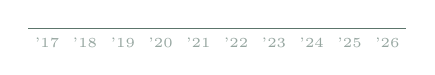
\begin{tikzpicture}[x=1mm,y=1mm]
    \pgfmathsetmacro\nyears{\the\year-\FirstPubYear+1}
    \pgfmathsetmacro\slot{48/\nyears}
    \pgfmathsetmacro\bw{0.62*\slot}
    \def\u{2.25}
    \draw[white!30!ink,line width=0.4pt] (0,0) -- (48,0);
    \foreach \y [count=\i from 0] in {\FirstPubYear,...,\the\year}{
      \pgfmathsetmacro\xa{\i*\slot+(\slot-\bw)/2}
      \pgfmathsetmacro\c{\PY{\y}{C}}\pgfmathsetmacro\j{\PY{\y}{J}}\pgfmathsetmacro\w{\PY{\y}{W}}
      \foreach \n/\col [remember=\top as \bot (initially 0)] in
          {\c/accentlight,\j/white!88!ink,\w/white!45!ink}{
        \pgfmathsetmacro\top{\bot+\n}
        \ifdim\n pt>0pt
          \fill[\col] (\xa,\bot*\u+0.35) rectangle ++(\bw,\n*\u-0.35);
        \fi}
      \pgfmathtruncatemacro\yy{mod(\y,100)}
      \node[font=\FiraBook\fontsize{5.5}{6}\selectfont,text=white!55!ink,anchor=north,inner sep=0pt]
        at (\xa+\bw/2,-1.1) {’\yy};}
  \end{tikzpicture}\par\vspace{2.2mm}%
  {\fontsize{6.5}{8}\selectfont\color{white!72!ink}%
   {\color{accentlight}\rule{1.8mm}{1.8mm}}\hspace{1mm}conference\hspace{2.2mm}%
   {\color{white!88!ink}\rule{1.8mm}{1.8mm}}\hspace{1mm}journal\hspace{2.2mm}%
   {\color{white!45!ink}\rule{1.8mm}{1.8mm}}\hspace{1mm}workshop}\par}
\newcommand{\sidechip}[1]{\tikz[baseline=(c.base)]\node[rounded corners=2pt,draw=white!40!ink,
  text=white!92!ink,font=\scriptsize,inner xsep=3pt,inner ysep=1.6pt] (c) {#1};}

% \showphotofalse

\begin{document}

%==============================================================================
%  PAGE 1  --  cover page with sidebar
%==============================================================================
\newgeometry{left=73mm,right=15mm,top=14mm,bottom=13mm,footskip=6mm}
\thispagestyle{cover}
\setlength\labelcol{16mm}\setlength\labelgap{4mm}\setlength\bodyindent{20mm}\setlength\entrysep{5pt}

\begin{tikzpicture}[remember picture,overlay]
  \fill[ink] (current page.north west) rectangle ([xshift=60mm]current page.south west);
  \fill[accent] ([xshift=60mm]current page.north west) rectangle ([xshift=61.2mm]current page.south west);
  % motif at the bottom of the sidebar: a finite model unravelled into a cactus
  % (after Figure 2 of "Towards Finite Satisfiability of PDL with Loops")
  \begin{scope}[shift={([xshift=30mm,yshift=30mm]current page.south west)},
      x=1mm,y=1mm,>={Stealth[length=1.6mm,width=1.3mm]},
      w/.style={circle,draw=#1,fill=#1!35!ink,line width=0.6pt,minimum size=3.4mm,inner sep=0pt,
                font=\FiraSemi\fontsize{5.5}{5.5}\selectfont,text=white},
      e/.style={->,line width=0.55pt,draw=white!45!ink},
      back/.style={->,line width=0.65pt,draw=gold,dash pattern=on 1.4pt off 1.1pt},
      tri/.style={fill=white!22!ink,draw=none},
      lab/.style={font=\fontsize{4.5}{4.5}\selectfont,text=white!50!ink,inner sep=0.6pt}]
    \colorlet{wa}{accentlight}\colorlet{wb}{gold}\definecolor{wc}{HTML}{E58C8A}
    % --- the finite model
    \node[w=wa] (a) at (-16.5,7) {a};
    \node[w=wb] (b) at (-11.5,-1.5) {b};
    \node[w=wc] (c) at (-21.5,-1.5) {c};
    \draw[e] (a) -- node[lab,right] {e} (b);
    \draw[e] (b) -- node[lab,below] {r} (c);
    \draw[e] (c) -- node[lab,left] {e} (a);
    \draw[e] (b) to[out=-30,in=-100,looseness=7] node[lab,below right=-0.5pt] {e} (b);
    % --- unravelling
    \draw[->,line width=0.6pt,draw=accentlight,decorate,
          decoration={snake,amplitude=0.55mm,segment length=2mm,post length=1.4mm}] (-8.2,2.5) -- (-3.6,2.5);
    % --- the cactus
    \node[w=wa] (r)  at (12,10) {a};
    \node[w=wb] (b1) at (4.5,2) {b};
    \node[w=wc] (c1) at (4.5,-6) {c};
    \node[w=wb] (b2) at (13,2) {b};
    \node[w=wb] (b3) at (13,-6) {b};
    \node[w=wc] (c2) at (20.5,2) {c};
    \draw[e] (r) -- (b1); \draw[e] (b1) -- (c1);
    \draw[e] (r) -- (b2); \draw[e] (b2) -- (b3);
    \draw[e] (r) -- (c2);
    \fill[tri] (c1.south) ++(0,-0.6) -- ++(-2.2,-4) -- ++(4.4,0) -- cycle;
    \fill[tri] (b3.south) ++(0,-0.6) -- ++(-2.2,-4) -- ++(4.4,0) -- cycle;
    \fill[tri] (c2.south) ++(0,-0.6) -- ++(-2.2,-4) -- ++(4.4,0) -- cycle;
    \draw[back] (c1.west) to[out=160,in=175,looseness=1.05] (r.west);
    \draw[back] (b3.east) to[out=40,in=-40,looseness=1.6] (b2.east);
    % --- caption
    \node[anchor=north,font=\FiraBook\fontsize{6}{7}\selectfont,text=white!55!ink,align=center]
      at (0,-13.2) {finite models\,\textrightarrow\,foldable cacti};
  \end{scope}
  \ifshowphoto
    \begin{scope}
      \clip ([xshift=30mm,yshift=-33mm]current page.north west) circle (18mm);
      \node at ([xshift=30mm,yshift=-33mm]current page.north west) {
\includegraphics[width=36.5mm]{photo.jpg}};
    \end{scope}
    \draw[accentlight,line width=1.1pt] ([xshift=30mm,yshift=-33mm]current page.north west) circle (18.5mm);
  \fi
  % sidebar content
  \node[anchor=north west,inner sep=0pt,text width=48mm,text=white!88!ink,font=\footnotesize]
    at ([xshift=6mm,yshift=-13mm]current page.north west) {%
    \ifshowphoto\vspace*{38mm}\fi
    \sidehead{Contact}
    \sideitem{\faEnvelope}{\href{mailto:\EmailA}{\color{white}\EmailA}}
    \vspace{-1.2mm}\hspace*{5.5mm}{\scriptsize\color{accentlight}preferred}\par\vspace{1.5mm}
    \sideitem{\faEnvelope[regular]}{\href{mailto:\EmailB}{\color{white}\EmailB}}
    \sideitem{\faGlobe}{\href{https://\Website}{\color{white}\Website}}
    \sideitem{\aiOrcid}{\href{https://orcid.org/\ORCID}{\color{white}\ORCID}}
    \sideitem{\aiGoogleScholar}{\href{\ScholarURL}{\color{white}Google Scholar}\hspace{4mm}%
      {\color{accentlight}\aidblp}\hspace{1.5mm}\href{\DBLPURL}{\color{white}DBLP}}
    \sidehead{Offices}
    \sideitem{\faMapMarker*}{{\FiraSemi\color{white}TU Wien Informatics}}
    \vspace{-1.3mm}\hspace*{5.5mm}\parbox[t]{40mm}{\scriptsize Favoritenstraße 9--11, Room HE0340\\1040 Vienna, Austria}\par\vspace{2.2mm}
    \sideitem{\faMapMarker*}{{\FiraSemi\color{white}University of Wrocław}}
    \vspace{-1.3mm}\hspace*{5.5mm}\parbox[t]{40mm}{\scriptsize Joliot-Curie 15, Room 324\\50-383 Wrocław, Poland}\par
    \sidehead{Publications}
    \sidepubs
    \sidehead{Research interests}
    {\linespread{1.5}\selectfont
    \sidechip{finite model theory} \sidechip{dynamic logics} \sidechip{PDL \& μ-calculus}
    \sidechip{decidable fragments of FO} \sidechip{description logics} \sidechip{automata \& games}
    \sidechip{computational complexity}\par}
  };
\end{tikzpicture}%
%------------------------------------------------------------------ name block
{\FiraLight\fontsize{25}{27}\selectfont\color{ink}\FirstName\ \MiddleName}\par\vspace{1mm}
{\FiraSemi\fontsize{38}{40}\selectfont\color{ink}\LastName}\par\vspace{2.5mm}
{\color{accent}\rule{16mm}{1.6pt}}\par\vspace{3mm}
{\FiraMedium\color{ink}Senior Postdoc \& PI of the FWF ESPRIT project FINGO}\,\muted{\textendash\ TU Wien}\par\vspace{0.6mm}
{\FiraMedium\color{ink}Assistant Professor}\,\muted{\textendash\ University of Wrocław}\par\vspace{5mm}

%---------------------------------------------------------------------- profile
{\linespread{1.18}\selectfont\raggedright
I am a logician working in \emph{applied dendrology}: most of my current research uses trees, cacti and
flowers for finite-model reasoning in dynamic logics (extensions of PDL, the modal μ-calculus, and more).
More broadly, I study the decidability and complexity of fragments of first-order logic (guarded,
fluted/ordered, forward and two-variable), description logics and temporal logics, as well as finite model
theory and the theory of computation.\par}
\vspace{4.5mm}

%------------------------------------------------------------------- highlights
\begin{tcolorbox}[enhanced,colback=tint,colframe=tint,arc=3pt,boxrule=0pt,
    left=4.5mm,right=4mm,top=3.5mm,bottom=3.5mm,before skip=0pt,after skip=0pt,
    borderline west={2.4pt}{0pt}{accent}]
  {\color{accent}\FiraSemi\scriptsize\addfontfeature{LetterSpace=12}HIGHLIGHTS}\par\vspace{2mm}
  \small\renewcommand{\arraystretch}{1.28}%
  \begin{tabular}{@{}c@{\hspace{3mm}}>{\raggedright\arraybackslash}p{0.88\linewidth}@{}}
    {\color{accent}\faCoins}          & PI of the \semi{FWF ESPRIT} project \semi{FINGO} at TU Wien (346\,505\,EUR)\\
    {\color{accent}\faGraduationCap}  & \semi{PhD with distinction}, TU Dresden (2024)\\
    {\color{gold}\faTrophy}           & \semi{Two Best Student Paper Awards} (JELIA 2021, JELIA 2023)\\
    {\color{gold}\faAward}            & \semi{Award for Outstanding Young Scientists}, Polish Ministry (2021)\\
    {\color{accent}\faBookOpen}       & Papers at \semi{LICS, ICALP, IJCAI, AAAI, KR}; articles in \semi{LMCS, JAIR, ToCL}\\
    {\color{accent}\faUserGraduate}   & \semi{\TotalThesis\ supervised theses}; supervising a PhD student since 2026\\
    {\color{accent}\faChalkboardTeacher} & \semi{Five-day course at ESSLLI 2026}, co-taught with Ian~Pratt-Hartmann
  \end{tabular}
\end{tcolorbox}

%==============================================================================
\cvsection{\faBriefcase}{Employment}
\begin{entries}
\entry{\range{04.2026}{03.2029}}{Senior Postdoc \& PI of FWF project FINGO}{TU Wien}
  {Institute of Logic and Computation; mentor: Magdalena~Ortiz.}
\entry{\range{03.2025}{03.2026}}{Postdoctoral Researcher (part-time)}{TU Wien}
  {FWF project \emph{ONTEGRA} (PI: Magdalena Ortiz).}
\entry{\range{10.2024}{present}}{Assistant Professor}{University of Wrocław}
  {Institute of Computer Science; currently on a 20\%~workload.}
\entry{\range{04.2019}{09.2024}}{Research Associate}{TU Dresden}
  {Computational Logic Group; ERC CoG \emph{DeciGUT} (PI: Sebastian Rudolph).}
\entry{\range{03.2017}{06.2018}}{Student Researcher}{University of Wrocław}
  {NCN grant \emph{A quest for new computer logics} (PI: Emanuel Kieroński).}
\end{entries}

%==============================================================================
\cvsection{\faGraduationCap}{Education}
\begin{entries}
\entry{\range{2019}{06.2024}}{PhD (Dr.\,rer.\,nat.), \emph{with distinction}\nobreak\hspace{0.35em}{\tiny\href{https://bartoszjanbednarczyk.github.io/others/phd-certificate.pdf}{\color{accent}\faExternalLink*}}}{TU Dresden}
  {\emph{\weblink{https://nbn-resolving.org/urn:nbn:de:bsz:14-qucosa2-925378}{Database-Inspired Reasoning Problems in Description Logics With Path~Expressions}}\nobreak\hspace{0.35em}\iconlink{https://bartoszjanbednarczyk.github.io/slides/Bednarczyk-PhD-Defense-Slides.pdf}{\faDesktop}\\
   Supervisors: S.~Rudolph, E.~Kieroński\sep reviewers: S.~Rudolph, M.~Ortiz}
\entry{\range{2017}{2018}}{M1 in Computer Science (MPRI)}{ENS Paris-Saclay}
  {\emph{Assertion Languages with Modalities and Separating Connectives}\nobreak\hspace{0.35em}\iconlink{https://bartoszjanbednarczyk.github.io/slides/MPRI2018-defense-slides.pdf}{\faDesktop}\\
   Supervisor: S.~Demri\sep \semi{magna cum laude}\sep published at LICS~2019}
\entry{\range{2014}{2017}}{BSc in Computer Science}{University of Wrocław}
  {\emph{\weblink{https://apd.uni.wroc.pl/diplomas/30417/}{Satisfiability of the Two-Variable Fragment of First-Order Logic with Counting Quantifiers over Finite~Trees}}\\
   Supervisor: W.~Charatonik\sep published at CSL~2017}
\end{entries}

\restoregeometry
\newpage
\setlength\labelcol{22mm}\setlength\labelgap{5mm}\setlength\bodyindent{27mm}\setlength\entrysep{5pt}
%==============================================================================
%  PAGE 2 ff.
%==============================================================================

\cvsection{\faStream}{Career at a glance}
\noindent\begin{tikzpicture}[x=9.6mm,y=1mm,
    bar/.style={rounded corners=2pt,fill=#1,draw=none},
    lbl/.style={text=white,font=\FiraSemi\scriptsize,inner sep=0pt},
    lane/.style={anchor=east,font=\FiraSemi\scriptsize,text=ink},
    mk/.style={font=\scriptsize,inner sep=0pt}]
  \begin{scope}[xshift=22mm]
  \foreach \y/\t in {0/Studies,-8/Positions,-24/Grants (PI),-40/Research stays,-48/Awards}
    {\node[lane] at (-0.35,\y) {\t};}
  \foreach \yr in {2014,...,2029}{
    \draw[hair,line width=0.4pt] ({\yr-2014},4) -- ({\yr-2014},-58);
    \node[font=\FiraBook\scriptsize,text=muted,anchor=north] at ({\yr-2014},-59.5) {\yr};}
  \draw[gold,line width=0.9pt,dashed] (12.76,6) -- (12.76,-58);
  \node[font=\FiraSemi\scriptsize,text=gold,anchor=south] at (12.76,6) {today};
  % studies
  \fill[bar=inksoft] (0.75,-2.8) rectangle (3.12,2.8);  \node[lbl] at (1.93,0) {BSc Wrocław};
  \fill[bar=inksoft] (3.70,-2.8) rectangle (4.70,2.8);  \node[lbl] at (4.20,0) {M1};
  \fill[bar=inksoft] (5.25,-2.8) rectangle (10.48,2.8); \node[lbl] at (7.86,0) {PhD, TU Dresden};
  % positions
  \fill[bar=accent] (3.17,-10.8) rectangle (4.50,-5.2);  \node[lbl] at (3.835,-8) {NCN};
  \fill[bar=accent] (5.25,-10.8) rectangle (10.73,-5.2); \node[lbl] at (7.99,-8) {Research Associate, TU Dresden};
  \fill[bar=accent] (11.17,-10.8) rectangle (12.23,-5.2);\node[lbl,font=\FiraSemi\tiny] at (11.70,-8) {Postdoc};
  \fill[bar=accent] (12.25,-10.8) rectangle (15.25,-5.2);\node[lbl] at (13.75,-8) {Senior Postdoc, TU Wien};
  \shade[left color=accent!70!ink,right color=white,rounded corners=2pt] (13.4,-18.8) rectangle (15.5,-13.2);
  \fill[accent!70!ink,rounded corners=2pt] (10.75,-18.8) rectangle (13.6,-13.2);
  \node[lbl] at (12.55,-16) {Assistant Professor, Wrocław};
  % grants
  \fill[bar=ink] (12.25,-26.8) rectangle (15.25,-21.2);\node[lbl] at (13.75,-24) {FWF ESPRIT FINGO};
  \fill[bar=ink] (11.0,-34.8) rectangle (13.0,-29.2);  \node[lbl] at (12.0,-32) {NCN Preludium};
  % research stays
  \foreach \x in {3.55,4.62,7.5}{\node[circle,fill=inksoft,inner sep=0pt,minimum size=2.6mm] at (\x,-40) {};}
  \node[mk,text=inksoft,anchor=east] at (3.38,-40) {IST Austria};
  \node[mk,text=inksoft,anchor=west] at (4.79,-40) {Oxford};
  \node[mk,text=inksoft,anchor=west] at (7.67,-40) {Tampere};
  % awards
  \foreach \x/\t/\y in {5.5/Steinhaus/-55,7.38/JELIA BSPA/-51.5,7.9/Ministry award/-55,9.7/JELIA BSPA/-51.5}{
    \node[text=gold,font=\small] at (\x,-48) {\faTrophy};
    \node[mk,text=gold,anchor=north] at (\x,\y) {\t};}
  \end{scope}
\end{tikzpicture}

%==============================================================================
\cvsection{\faCoins}{Research funding}
\cvsubsection{As principal investigator}
\grantcard[https://www.fwf.ac.at/en/research-radar/10.55776/ESP2407425]{\range{04.2026}{03.2029}}
  {FINGO: Finite Graph Operating Automata Meet Dynamic Logics}
  {FWF ESPRIT grant, Austrian Science Fund}
  {Hosted by TU Wien\sep DOI \href{https://www.fwf.ac.at/en/research-radar/10.55776/ESP2407425}{10.55776/ESP2407425}\\
   Finite-model reasoning for extensions of PDL and the μ-calculus.}
  {346\,505 EUR}{36 months}
\grantcard{\range{01.2025}{12.2026}}
  {Decision Problems for Logics with Weak Forms of Recursion}
  {NCN Preludium grant, National Science Centre, Poland}
  {Hosted by the University of Wrocław\sep 2024/53/N/ST6/01390\\
   Ranked \semi{first} among all computer-science proposals.\\
   No-cost one-year extension; runs until December~2026.}
  {63\,600 PLN}{12 months, extended to 24}
\cvsubsection{As researcher}
\begin{entries}
\entry{\range{03.2025}{03.2026}}{\weblink{https://www.fwf.ac.at/en/research-radar/10.55776/PIN8884924}{FWF project ONTEGRA}}{TU Wien}
  {\emph{Ontology-based access to Temporal and Graph Data}\\PI: Magdalena Ortiz\sep 10.55776/PIN8884924}
\entry{\range{04.2019}{09.2024}}{\weblink{https://cordis.europa.eu/project/id/771779}{ERC Consolidator Grant DeciGUT}}{TU Dresden}
  {\emph{A Grand Unified Theory of Decidability in Logic-Based Knowledge Representation}\\PI: Sebastian Rudolph\sep grant agreement 771779}
\entry{\range{03.2017}{06.2018}}{NCN Opus grant}{University of Wrocław}
  {\emph{A quest for new computer logics}\\PI: Emanuel Kieroński\sep 2016/21/B/ST6/01444}
\end{entries}

%==============================================================================
\cvsection{\faTrophy}{Awards \& honours}
\begin{entries}
\entry{2025}{Nomination for the GI Dissertationspreis}{Gesellschaft für Informatik}
  {Annual award of the German Informatics Society for the best PhD thesis in computer science.\\
   Nomination declined.}
\entry{2023}{\weblink{https://bartoszjanbednarczyk.github.io/others/JELIA2023_award_signed.pdf}{Best Student Paper Award, JELIA 2023}}{500 EUR\sep unrestricted use}
  {For \emph{Beyond ALCreg: Exploring Non-Regular Extensions of PDL with Description Logics~Features}.}
\entry{2021}{Award for Outstanding Young Scientists}{194\,040 PLN\sep unrestricted use}
  {Polish Ministry of Science and Higher Education.}
\entry{2021}{\weblink{https://bartoszjanbednarczyk.github.io/others/JELIA2021_BSPA_Bednarczyk.pdf}{Best Student Paper Award, JELIA 2021}}{500 EUR\sep unrestricted use}
  {For \emph{Exploiting Forwardness: Satisfiability and Query-Entailment in Forward Guarded~Fragment}.}
\entry{2019}{Hugo Steinhaus Scholarship for Mathematical Sciences}{18\,000 PLN\sep unrestricted use}
  {Awarded to outstanding PhD students in Wrocław.}
\end{entries}

%==============================================================================
\cvsection{\faGlobeEurope}{Longer research stays}
\begin{entries}
\entry{2021}{Tampere University, Finland}{2 months}{Model theory of ordered logics.\ Host: Antti Kuusisto.}
\entry{2018}{TU Dresden, Germany}{weekly visits over $\approx$\,6 months}{Query entailment in description logics.\ Host: Sebastian Rudolph.}
\entry{2018}{University of Oxford, United Kingdom}{3-month internship}
  {Tree algebras and their connections to circuit complexity.\ Hosts: James Worrell and Michaël Cadilhac.}
\entry{2017}{IST Austria, Klosterneuburg}{3-month internship}
  {Temporal logics for quantitative properties and weighted automata.\ Host: Krishnendu Chatterjee.}
\end{entries}

%==============================================================================
\cvsection{\faLaptopCode}{Industry experience}
\begin{entries}
\entry{during studies}{Software Engineering Intern}{Bloomberg, London}{Monitoring Cassandra databases (3~months).}
\entry{during studies}{Software Engineering Intern}{Neurosoft, Wrocław}{Developing web applications with Groovy and MongoDB (3~months).}
\end{entries}

%==============================================================================
\cvsection{\faBookOpen}{Publications}
\hspace*{\bodyindent}\parbox{\dimexpr\linewidth-\bodyindent\relax}{\small\color{muted}%
\cvtag[typeJ]{J}~journal\quad\cvtag[typeC]{C}~conference\quad\cvtag[typeW]{W}~workshop / student session\quad
\cvtag[typeT]{T}~thesis\hfill abstracts on \href{https://\Website/publications.html}{my website}\\[1pt]
Titles link to the publisher's page;\quad {\color{accent}\faFilePdf[regular]}~PDF\quad {\color{accent}\faDesktop}~slides\quad
{\color{accent}\faVideo}~video\quad {\color{accent}\tiny\faExternalLink*}~external page}\par

\cvsubsection{Under submission}
\begin{publist}
\preprint{Towards Finite Satisfiability of PDL with Loops}{Mikołaj Swoboda}
\preprint{Two Variables and Two-Dimensional Structures}{Daumantas Kojelis, Krzysztof Szymański}
\end{publist}

\cvsubsection{Journal articles}
\begin{publist}
\pub[url=https://doi.org/10.1093/logcom/exaf042, pdf=https://iccl.inf.tu-dresden.de/w/images/2/2c/Adjacent-fragment.pdf]{J}{JLC}{2025}{The Adjacent Fragment and Quine's Limits of Decision}
  {Daumantas Kojelis, Ian Pratt-Hartmann}{Journal of Logic and Computation}{}
\pub[url=https://lmcs.episciences.org/15442, pdf=https://lmcs.episciences.org/15442/pdf]{J}{LMCS}{2025}{About the Expressive Power and Complexity of Order-Invariance with Two Variables}
  {Julien Grange}{Logical Methods in Computer Science}{}
\pub[url=https://lmcs.episciences.org/13581, pdf=https://lmcs.episciences.org/13581/pdf]{J}{LMCS}{2024}{Exploring Non-Regular Extensions of Propositional Dynamic Logic with Description-Logics Features}
  {}{Logical Methods in Computer Science}{}
\pub[url=https://jair.org/index.php/jair/article/view/14482, pdf=https://jair.org/index.php/jair/article/view/14482/26975]{J}{JAIR}{2023}{How to Tell Easy from Hard: Complexity of Conjunctive Query Entailment in Extensions of ALC}
  {Sebastian Rudolph}{Journal of Artificial Intelligence Research}{}
\pub[url=https://doi.org/10.1145/3569954, pdf=https://dl.acm.org/doi/pdf/10.1145/3569954]{J}{ToCL}{2023}{On Composing Finite Forests with Modal Logics}
  {Stéphane Demri, Raul Fervari, Alessio Mansutti}{ACM Transactions on Computational Logic}{}
\pub[url=https://lmcs.episciences.org/9849, pdf=https://lmcs.episciences.org/9849/pdf]{J}{LMCS}{2022}{Why Does Propositional Quantification Make Modal and Temporal Logics on Trees Robustly Hard?}
  {Stéphane Demri}{Logical Methods in Computer Science}{}
\pub[url=https://doi.org/10.1017/S1471068421000065, pdf=https://arxiv.org/pdf/1812.04413]{J}{TPLP}{2021}{Completing the Picture: Complexity of Graded Modal Logics with Converse}
  {Emanuel Kieroński, Piotr Witkowski}{Theory and Practice of Logic Programming}{\cvtag[ink]{invited}}
\pub[url=https://doi.org/10.1016/j.ipl.2021.106113, pdf=https://arxiv.org/pdf/1911.00696]{J}{IPL}{2021}{Statistical EL is ExpTime-complete}
  {}{Information Processing Letters}{}
\pub[url=https://doi.org/10.1016/j.tcs.2019.09.028, pdf=https://arxiv.org/pdf/1810.10899]{J}{TCS}{2020}{One-Variable Logic Meets Presburger Arithmetic}
  {}{Theoretical Computer Science}{}
\end{publist}

\cvsubsection{Peer-reviewed conference papers}
\begin{publist}
\pub[url=https://doi.org/10.24963/kr.2025/9, pdf=https://arxiv.org/pdf/2509.09218, slides=https://bartoszjanbednarczyk.github.io/slides/Bednarczyk-KR2025.pdf]{C}{KR}{2025}{Guarded Fragments Meet Dynamic Logic: The Story of Regular Guards}
  {Emanuel Kieroński}{Principles of Knowledge Representation and Reasoning (KR 2025)}{}
\pub[url=https://www.ijcai.org/proceedings/2024/359, pdf=https://www.ijcai.org/proceedings/2024/0359.pdf, slides=https://bartoszjanbednarczyk.github.io/slides/IJCAI2024-long.pdf]{C}{IJCAI}{2024}{Data Complexity in Expressive Description Logics With Path Expressions}
  {}{Int.\ Joint Conference on Artificial Intelligence (IJCAI 2024)}{}
\pub[url=https://doi.org/10.1007/978-3-031-43619-2_21, pdf=https://iccl.inf.tu-dresden.de/w/images/d/d2/BBE-JELIA23-FINAL.pdf, slides=https://bartoszjanbednarczyk.github.io/slides/JELIA2023-slides.pdf]{C}{JELIA}{2023}{Beyond ALCreg: Exploring Non-Regular Extensions of PDL with Description Logics Features}
  {}{European Conference on Logics in Artificial Intelligence (JELIA 2023)}{\bestpaper}
\pub[url=https://doi.org/10.4230/LIPIcs.ICALP.2023.111, pdf=https://iccl.inf.tu-dresden.de/w/images/6/69/BBE-ICALP23-Corrected.pdf]{C}{ICALP}{2023}{On the Limits of Decision: the Adjacent Fragment of First-Order Logic}
  {Daumantas Kojelis, Ian Pratt-Hartmann}{Int.\ Colloquium on Automata, Languages and Programming (ICALP 2023)}{}
\pub[url=https://doi.org/10.1007/978-3-031-15298-6_19, pdf=https://iccl.inf.tu-dresden.de/w/images/e/e7/Wollic2022-paper-34.pdf]{C}{WoLLIC}{2022}{Presburger Büchi Tree Automata with Applications to Logics with Expressive Counting}
  {Oskar Fiuk}{Logic, Language, Information and Computation (WoLLIC 2022)}{}
\pub[url=https://doi.org/10.4230/LIPIcs.MFCS.2022.15, pdf=https://drops.dagstuhl.de/opus/volltexte/2022/16813/pdf/LIPIcs-MFCS-2022-15.pdf, slides=https://bartoszjanbednarczyk.github.io/slides/MFCS2022-MTofOrderedFragments.pdf]{C}{MFCS}{2022}{Towards Model Theory of Ordered Logics: Expressivity and Interpolation}
  {Reijo Jaakkola}{Mathematical Foundations of Computer Science (MFCS 2022)}{}
\pub[url=https://ojs.aaai.org/index.php/AAAI/article/view/20487, pdf=https://ojs.aaai.org/index.php/AAAI/article/view/20487/20246, slides=https://bartoszjanbednarczyk.github.io/slides/AAAI2022-ZOIQ-long.pdf]{C}{AAAI}{2022}{Finite Entailment of Local Queries in the Z Family of Description Logics}
  {Emanuel Kieroński}{AAAI Conference on Artificial Intelligence (AAAI 2022)}{}
\pub[url=https://ojs.aaai.org/index.php/AAAI/article/view/20488, pdf=https://ojs.aaai.org/index.php/AAAI/article/view/20488/20247, slides=https://bartoszjanbednarczyk.github.io/slides/AAAI2022-ALCSelf-long.pdf]{C}{AAAI}{2022}{The Price of Selfishness: Conjunctive Query Entailment for ALCSelf is 2ExpTime-hard}
  {Sebastian Rudolph}{AAAI Conference on Artificial Intelligence (AAAI 2022)}{}
\pub[url=https://doi.org/10.4230/LIPIcs.FSTTCS.2021.36, pdf=https://iccl.inf.tu-dresden.de/w/images/1/14/Bednarczyk-FSTTCS2021.pdf, slides=https://bartoszjanbednarczyk.github.io/slides/FSTTCS2021-slides.pdf, video=https://bartoszjanbednarczyk.github.io/slides/FSTTCS2021-video.mp4]{C}{FSTTCS}{2021}{On Classical Decidable Logics Extended with Percentage Quantifiers and Arithmetics}
  {Maja Orłowska, Anna Pacanowska, Tony Tan}{Foundations of Software Technology and Theoretical Computer Science (FSTTCS 2021)}{}
\pub[url=https://doi.org/10.1007/978-3-030-75775-5_13, pdf=https://iccl.inf.tu-dresden.de/w/images/e/e6/Jelia2021-bbe.pdf, slides=https://bartoszjanbednarczyk.github.io/slides/JELIA2021-slides.pdf]{C}{JELIA}{2021}{Exploiting Forwardness: Satisfiability and Query-Entailment in Forward Guarded Fragment}
  {}{European Conference on Logics in Artificial Intelligence (JELIA 2021)}{\bestpaper}
\pub[url=https://doi.org/10.1007/978-3-030-71995-1_5, pdf=https://arxiv.org/pdf/2007.01233, slides=https://bartoszjanbednarczyk.github.io/slides/FOSSACS2021-slides.pdf, video=https://bartoszjanbednarczyk.github.io/slides/FOSSACS2021-video.mp4]{C}{FoSSaCS}{2021}{``Most of'' Leads to Undecidability: Failure of Adding Frequencies to LTL}
  {Jakub Michaliszyn}{Foundations of Software Science and Computation Structures (FoSSaCS 2021)}{}
\pub[url=https://doi.org/10.4230/LIPIcs.TIME.2020.17]{C}{TIME}{2020}{A Note on C\textsuperscript{2} Interpreted over Finite Data-Words}
  {Piotr Witkowski}{Temporal Representation and Reasoning (TIME 2020)}{}
\pub[url=https://www.ijcai.org/Proceedings/2020/238, pdf=https://www.ijcai.org/Proceedings/2020/0238.pdf]{C}{IJCAI}{2020}{All-Instances Oblivious Chase Termination is Undecidable for Single-Head Binary TGDs}
  {Robert Ferens, Piotr Ostropolski-Nalewaja}{Int.\ Joint Conference on Artificial Intelligence (IJCAI-PRICAI 2020)}{}
\pub[url=https://www.ijcai.org/Proceedings/2020/233, pdf=https://www.ijcai.org/Proceedings/2020/0233.pdf, slides=https://bartoszjanbednarczyk.github.io/slides/IJCAI20-DL-slides.pdf, video=https://bartoszjanbednarczyk.github.io/slides/IJCAI20-DL-video.mp4]{C}{IJCAI}{2020}{A Framework for Reasoning about Dynamic Axioms in Description Logics}
  {Stéphane Demri, Alessio Mansutti}{Int.\ Joint Conference on Artificial Intelligence (IJCAI-PRICAI 2020)}{}
\pub[url=https://doi.org/10.1145/3373718.3394787, pdf=http://www.lsv.fr/Publis/PAPERS/PDF/BDFM-lics2020.pdf, video={https://www.youtube.com/watch?v=lviuGYX6_9k}]{C}{LICS}{2020}{Modal Logics with Composition on Finite Forests: Expressivity and Complexity}
  {Stéphane Demri, Raul Fervari, Alessio Mansutti}{ACM/IEEE Symposium on Logic in Computer Science (LICS 2020)}{}
\pub[url=https://ebooks.iospress.nl/publication/54941, pdf=https://arxiv.org/pdf/2002.06072, slides=https://bartoszjanbednarczyk.github.io/slides/ECAI2020-slides.pdf, video=https://bartoszjanbednarczyk.github.io/slides/ECAI2020-video.mov]{C}{ECAI}{2020}{Satisfiability and Query Answering in Description Logics with Global and Local Cardinality Constraints}
  {Franz Baader, Sebastian Rudolph}{European Conference on Artificial Intelligence (ECAI 2020)}{}
\pub[url=https://www.ijcai.org/proceedings/2019/212, pdf=https://www.ijcai.org/proceedings/2019/0212.pdf, slides=https://bartoszjanbednarczyk.github.io/slides/IJCAI2019-slides.pdf]{C}{IJCAI}{2019}{Worst-Case Optimal Querying of Very Expressive Description Logics with Path Expressions and Succinct Counting}
  {Sebastian Rudolph}{Int.\ Joint Conference on Artificial Intelligence (IJCAI 2019)}{}
\pub[url=https://ieeexplore.ieee.org/document/8785656, pdf=http://www.lsv.fr/Publis/PAPERS/PDF/BD-lics2019.pdf, slides=https://bartoszjanbednarczyk.github.io/slides/LICS2019-slides.pdf]{C}{LICS}{2019}{Why Propositional Quantification Makes Modal Logics on Trees Robustly Hard?}
  {Stéphane Demri}{ACM/IEEE Symposium on Logic in Computer Science (LICS 2019)}{}
\pub[url=https://doi.org/10.1007/978-3-030-19570-0_42, pdf=https://arxiv.org/pdf/1812.04413]{C}{JELIA}{2019}{On the Complexity of Graded Modal Logics with Converse}
  {Emanuel Kieroński, Piotr Witkowski}{European Conference on Logics in Artificial Intelligence (JELIA 2019)}{}
\pub[url=https://doi.org/10.4230/LIPIcs.FSTTCS.2017.12, pdf=https://drops.dagstuhl.de/opus/volltexte/2018/8408/pdf/LIPIcs-FSTTCS-2017-12.pdf, slides=https://bartoszjanbednarczyk.github.io/slides/FSTTCS2017-slides.pdf]{C}{FSTTCS}{2017}{Modulo Counting on Words and Trees}
  {Witold Charatonik}{Foundations of Software Technology and Theoretical Computer Science (FSTTCS 2017)}{}
\pub[url=https://doi.org/10.4230/LIPIcs.CSL.2017.11, pdf=https://drops.dagstuhl.de/opus/volltexte/2017/7679/pdf/LIPIcs-CSL-2017-11.pdf, slides=https://bartoszjanbednarczyk.github.io/slides/CSL2017-slides.pdf]{C}{CSL}{2017}{Extending Two-Variable Logic on Trees}
  {Witold Charatonik, Emanuel Kieroński}{EACSL Annual Conference on Computer Science Logic (CSL 2017)}{}
\end{publist}

\cvsubsection{Workshop papers \& student sessions}
\begin{publist}
\pub[url=https://ceur-ws.org/Vol-4230/, pdf=https://ceur-ws.org/Vol-4230/dl-paper30.pdf]{W}{DL}{2026}{Baby Steps Towards Finite Satisfiability for LoopPDL}
  {Mikołaj Swoboda}{Int.\ Workshop on Description Logics (DL 2026)}{}
\pub[url=https://ceur-ws.org/Vol-4230/, pdf=https://ceur-ws.org/Vol-4230/dl-paper35.pdf]{W}{DL}{2026}{A Horn Extension of DL-Lite with NL Data Complexity}
  {Janos Arpasi, Magdalena Ortiz}{Int.\ Workshop on Description Logics (DL 2026)}{}
\pub[url=https://ceur-ws.org/Vol-4091/, pdf=https://ceur-ws.org/Vol-4091/paper09.pdf]{W}{DL}{2025}{Guarded Fragments Meet Dynamic Logic: The Story of Regular Guards (Extended Abstract)}
  {Emanuel Kieroński}{Int.\ Workshop on Description Logics (DL 2025)}{}
\pub[url=https://ceur-ws.org/Vol-3739/, pdf=https://ceur-ws.org/Vol-3739/abstract-6.pdf]{W}{DL}{2024}{Data Complexity in Expressive Description Logics With Path Expressions (Extended Abstract)}
  {}{Int.\ Workshop on Description Logics (DL 2024)}{}
\pub[url=https://ceur-ws.org/Vol-3739/, pdf=https://ceur-ws.org/Vol-3739/abstract-7.pdf]{W}{DL}{2024}{On the Limits of Decision: the Adjacent Fragment of First-Order Logic (Extended Abstract)}
  {Daumantas Kojelis, Ian Pratt-Hartmann}{Int.\ Workshop on Description Logics (DL 2024)}{}
\pub[pdf=https://iccl.inf.tu-dresden.de/w/images/6/66/Comonadic.pdf]{W}{DL}{2022}{Comonadic Semantics for Description Logics Games}
  {Mateusz Urbańczyk}{Int.\ Workshop on Description Logics (DL 2022)}{}
\pub[url=https://arxiv.org/abs/2106.15150, pdf=https://iccl.inf.tu-dresden.de/w/images/0/08/DL2021-Alcself.pdf, slides=https://bartoszjanbednarczyk.github.io/slides/DL2021-ALCSelf-slides.pdf]{W}{DL}{2021}{The Price of Selfishness: Conjunctive Query Entailment for ALCSelf is 2ExpTime-hard (Extended Abstract)}
  {Sebastian Rudolph}{Int.\ Workshop on Description Logics (DL 2021)}{}
\pub[pdf=https://iccl.inf.tu-dresden.de/w/images/8/82/DL2021-Z.pdf, slides=https://bartoszjanbednarczyk.github.io/slides/DL2021-ZOIQ-slides.pdf]{W}{DL}{2021}{Finite-Controllability of Conjunctive Queries in the Z Family of Description Logics (Extended Abstract)}
  {Emanuel Kieroński}{Int.\ Workshop on Description Logics (DL 2021)}{}
\pub[url=https://ceur-ws.org/Vol-2373/, pdf=https://ceur-ws.org/Vol-2373/paper-4.pdf, slides=https://bartoszjanbednarczyk.github.io/slides/IJCAI2019-slides.pdf]{W}{DL}{2019}{Worst-Case Optimal Querying of Very Expressive Description Logics with Path Expressions and Succinct Counting}
  {Sebastian Rudolph}{Int.\ Workshop on Description Logics (DL 2019)}{}
\pub[url=https://ceur-ws.org/Vol-2373/, pdf=https://ceur-ws.org/Vol-2373/paper-3.pdf, slides=https://bartoszjanbednarczyk.github.io/slides/DL2019-ALCSCC-slides.pdf]{W}{DL}{2019}{Satisfiability Checking and Conjunctive Query Answering in Description Logics with Global and Local Cardinality Constraints}
  {Franz Baader, Sebastian Rudolph}{Int.\ Workshop on Description Logics (DL 2019)}{}
\pub[url=http://www2.sfs.uni-tuebingen.de/esslli-stus-2017/, pdf=http://www2.sfs.uni-tuebingen.de/esslli-stus-2017/preproceedings_stus_2017.pdf, slides=https://bartoszjanbednarczyk.github.io/slides/ESSLLI2017-slides.pdf]{W}{ESSLLI}{2017}{On One Variable Fragment of First Order Logic with Modulo Counting Quantifier}
  {}{ESSLLI 2017 Student Session}{}
\end{publist}

\cvsubsection{Theses}
\begin{publist}
\pub[url=https://nbn-resolving.org/urn:nbn:de:bsz:14-qucosa2-925378, pdf=https://bartoszjanbednarczyk.github.io/others/PhD-thesis-Bednarczyk-2024.pdf, slides=https://bartoszjanbednarczyk.github.io/slides/Bednarczyk-PhD-Defense-Slides.pdf]{T}{PhD}{2024}{Database-Inspired Reasoning Problems in Description Logics With Path Expressions}
  {}{Doctoral thesis, TU Dresden (with distinction)}{}
\pub[pdf=https://bartoszjanbednarczyk.github.io/others/MPRI2018-thesis-Bednarczyk.pdf, slides=https://bartoszjanbednarczyk.github.io/slides/MPRI2018-defense-slides.pdf]{T}{M1}{2018}{Assertion Languages with Modalities and Separating Connectives}
  {}{M1 thesis (MPRI), ENS Paris-Saclay; supervisor: S.~Demri; defended in Cachan, 07.09.2018}{}
\pub[url=https://apd.uni.wroc.pl/diplomas/30417/, pdf=https://bartoszjanbednarczyk.github.io/others/BSc-thesis-Bednarczyk-2017.pdf]{T}{BSc}{2017}{Satisfiability of the Two-Variable Fragment of First-Order Logic with Counting Quantifiers over Finite Trees}
  {}{Bachelor thesis, University of Wrocław}{}
\end{publist}

%==============================================================================
\cvsection{\faMicrophone}{Talks}
\begin{stripedtable}{17mm}{42mm}{100mm}{}
\rowcolor{ink}\colhead{Date} & \colhead{Event} & \colhead{Title}\\
\endfirsthead
\rowcolor{ink}\colhead{Date} & \colhead{Event} & \colhead{Title}\\
\endhead
\talk[slides=https://bartoszjanbednarczyk.github.io/slides/Bednarczyk-KR2025.pdf]{11.2025}{KR 2025}{Melbourne, Australia}{Guarded Fragments Meet Dynamic Logic: The Story of Regular Guards}
\talk{05.09.2025}{DL 2025}{Opole, Poland}{Guarded Fragments Meet Dynamic Logic: The Story of Regular Guards}
\talk{30.05.2025}{FMT 2025 \cvtag{workshop}}{Finite and Algorithmic Model Theory, Les Houches, France}{Guarded Fragments Meet Dynamic Logic: The Story of Regular Guards}
\talk[slides=https://bartoszjanbednarczyk.github.io/slides/IJCAI2024-long.pdf]{08.2024}{IJCAI 2024}{Jeju, South Korea}{Data Complexity in Expressive Description Logics With Path Expressions}
\talk{06.2024}{DL 2024}{Bergen, Norway}{Data Complexity in Expressive Description Logics With Path Expressions}
\talk[slides=https://bartoszjanbednarczyk.github.io/slides/JELIA2023-slides.pdf]{09.2023}{JELIA 2023}{Dresden, Germany}{Beyond ALCreg: Exploring Non-Regular Extensions of PDL with Description Logics Features}
\talk{04.09.2023}{DL 2023}{Rhodes, Greece}{Undecidability Results for Non-Regular Extensions of ALCreg with Description-Logics Features}
\talk{03.03.2023}{AlMoTh 2023 \cvtag{workshop}}{Algorithmic Model Theory Meeting, Bochum, Germany}{Forward Guarded Fragment: A Tamed Higher-Arity Extension of Modal and Description Logics}
\talk[slides=https://bartoszjanbednarczyk.github.io/slides/MFCS2022-MTofOrderedFragments.pdf]{08.2022}{MFCS 2022}{Vienna, Austria}{Towards Model Theory of Ordered Logics: Expressivity and Interpolation}
\talk{31.07.2022}{DecFOML 2022 \cvtag{workshop}}{LICS workshop at FLoC, Haifa, Israel}{Forward Guarded Fragment: A Tamed Higher-Arity Extension of ALC}
\talk[slides=https://bartoszjanbednarczyk.github.io/slides/AAAI2022-ZOIQ-long.pdf]{02.2022}{AAAI 2022}{online}{Finite Entailment of Local Queries in the Z Family of Description Logics}
\talk[slides=https://bartoszjanbednarczyk.github.io/slides/AAAI2022-ALCSelf-long.pdf]{02.2022}{AAAI 2022}{online}{The Price of Selfishness: Conjunctive Query Entailment for ALCSelf is 2ExpTime-hard}
\talk[slides=https://bartoszjanbednarczyk.github.io/slides/DL2021-ALCSelf-slides.pdf]{09.2021}{DL 2021}{online}{The Price of Selfishness: Conjunctive Query Entailment for ALCSelf is 2ExpTime-hard}
\talk[slides=https://bartoszjanbednarczyk.github.io/slides/DL2021-ZOIQ-slides.pdf]{09.2021}{DL 2021}{online}{Finite-Controllability of Conjunctive Queries in the Z Family of Description Logics}
\talk[slides=https://bartoszjanbednarczyk.github.io/slides/QuantLA2021-slides.pdf]{22.06.2021}{QuantLA Seminar \cvtag{seminar}}{TU Dresden \& Leipzig University}{A Tamed Higher-Arity Extension of ALC: Forward Guarded Fragment}
\talk[slides=https://bartoszjanbednarczyk.github.io/slides/JELIA2021-slides.pdf]{17.05.2021}{JELIA 2021}{online}{Exploiting Forwardness: Satisfiability and Query-Entailment in Forward Guarded Fragment}
\talk[slides=https://bartoszjanbednarczyk.github.io/slides/FOSSACS2021-slides.pdf, video=https://bartoszjanbednarczyk.github.io/slides/FOSSACS2021-video.mp4]{03.2021}{FoSSaCS 2021}{ETAPS, online}{``Most of'' Leads to Undecidability: Failure of Adding Frequencies to LTL}
\talk[slides=https://bartoszjanbednarczyk.github.io/slides/IJCAI20-DL-slides.pdf, video=https://bartoszjanbednarczyk.github.io/slides/IJCAI20-DL-video.mp4]{13.01.2021}{IJCAI-PRICAI 2020}{online}{A Framework for Reasoning about Dynamic Axioms in Description Logics}
\talk{24.09.2020}{TIME 2020}{online}{A Note on C\textsuperscript{2} Interpreted over Finite Data-Words}
\talk[slides=https://bartoszjanbednarczyk.github.io/slides/ECAI2020-slides.pdf, video=https://bartoszjanbednarczyk.github.io/slides/ECAI2020-video.mov]{02.09.2020}{ECAI 2020}{online}{Satisfiability and Query Answering in Description Logics with Global and Local Cardinality Constraints}
\talk[slides=https://bartoszjanbednarczyk.github.io/slides/IJCAI2019-slides.pdf]{15.08.2019}{IJCAI 2019}{Macao, China}{Worst-Case Optimal Querying of Very Expressive Description Logics with Path Expressions and Succinct Counting}
\talk[slides=https://bartoszjanbednarczyk.github.io/slides/LICS2019-slides.pdf]{26.06.2019}{LICS 2019}{Vancouver, Canada}{Why Propositional Quantification Makes Modal Logics on Trees Robustly Hard?}
\talk[slides=https://bartoszjanbednarczyk.github.io/slides/DL2019-ALCSCC-slides.pdf]{20.06.2019}{DL 2019}{Oslo, Norway}{Satisfiability Checking and Conjunctive Query Answering in Description Logics with Global and Local Cardinality Constraints}
\talk[slides=https://bartoszjanbednarczyk.github.io/slides/IJCAI2019-slides.pdf]{18.06.2019}{DL 2019}{Oslo, Norway}{Worst-Case Optimal Querying of Very Expressive Description Logics with Path Expressions and Succinct Counting}
\talk{08.05.2019}{JELIA 2019}{Rende, Italy}{On the Complexity of Graded Modal Logics with Converse}
\talk[slides=https://bartoszjanbednarczyk.github.io/slides/FSTTCS2017-slides.pdf]{12.2017}{FSTTCS 2017}{Kanpur, India}{Modulo Counting on Words and Trees}
\talk[slides=https://bartoszjanbednarczyk.github.io/slides/CSL2017-slides.pdf]{08.2017}{CSL 2017}{Stockholm, Sweden}{Extending Two-Variable Logic on Trees}
\talk[slides=https://bartoszjanbednarczyk.github.io/slides/ESSLLI2017-slides.pdf]{07.2017}{\href{https://web.archive.org/web/20180526174105/http://www2.sfs.uni-tuebingen.de/esslli-stus-2017/}{\color{ink}ESSLLI 2017} \cvtag{student session}}{Toulouse, France}{On One Variable Fragment of First Order Logic with Modulo Counting Quantifier}
\end{stripedtable}

%==============================================================================
\cvsection{\faUserGraduate}{Student supervision}
\hspace*{\bodyindent}\parbox{\dimexpr\linewidth-\bodyindent\relax}{\small I supervise ambitious students, teach them
how to do research, and often write joint papers with them. Their theses led to publications at \semi{FSTTCS 2021},
\semi{WoLLIC 2022}, \semi{DL 2022} and \semi{DL~2026}.\par\vspace{2pt}
{\footnotesize\color{muted}\formalsup\,Officially registered under another supervisor, as I had no PhD yet; I supervised these theses in~full.}}\par\vspace{4mm}
\begin{stripedtable}{17mm}{50mm}{92mm}{}
\rowcolor{ink}\colhead{Year} & \colhead{Student} & \colhead{Thesis}\\
\endfirsthead
\rowcolor{ink}\colhead{Year} & \colhead{Student} & \colhead{Thesis}\\
\endhead
\leavevmode{\datefont since 2026} & \leavevmode{\FiraSemi\small\color{ink}Mikołaj Swoboda}\newline{\scriptsize\color{muted}PhD\sep University of Wrocław} & \leavevmode{\small\itshape PhD studies, ongoing}\\
\leavevmode{\datefont ongoing} & \leavevmode{\FiraSemi\small\color{ink}Christoph Schicha}\newline{\scriptsize\color{muted}BSc\sep TU Wien} & \leavevmode{\small\itshape Counting Automata and Temporal Domination}\\
\student[url=https://apd.uwr.edu.pl/diplomas/86023/]{2026}{Krzysztof Szymański}{BSc}{Univ.\ of Wrocław}{Finite Satisfiability Problem for Two-Variable Logic with One Successor and One Linear Order}{}
\student[url=https://apd.uwr.edu.pl/diplomas/86005/]{2026}{Michał Mądrala}{BSc}{Univ.\ of Wrocław}{On the Complexity of Forward Guarded Fragment with Constants}{}
\student[url=https://apd.uwr.edu.pl/diplomas/81587/]{2026}{Mikołaj Drozd}{BEng}{Univ.\ of Wrocław}{An application for visualizing games on finite graphs, with emphasis on Ehrenfeucht--Fraïssé games}{}
\student[url=https://apd.uwr.edu.pl/diplomas/79486/]{2026}{Mikołaj Swoboda}{MSc}{Univ.\ of Wrocław}{Finite Satisfiability Problem for Looping-PDL}{DL 2026}
\student[url=https://apd.uwr.edu.pl/diplomas/83781/]{2026}{Jadwiga Świerczyńska}{MSc}{Univ.\ of Wrocław}{Decidability of satisfiability for non-regular extensions of PDL}{}
\student[url=https://apd.uwr.edu.pl/diplomas/84840/]{2026}{Joanna Suwaj}{BSc}{Univ.\ of Wrocław}{Temporal Reasoning Through the Lens of Conjunctive Grammars}{}
\student[url=https://apd.uwr.edu.pl/diplomas/73813/]{2025}{Sebastian Zięciak}{MSc}{Univ.\ of Wrocław}{Towards Finite Controllability of Forward Sets of Existential Rules}{}
\leavevmode{\datefont 2025} & \leavevmode{\FiraSemi\small\color{ink}Tristan Parcollet}\newline{\scriptsize\color{muted}M1 internship\sep ENS Paris-Saclay} & \leavevmode{\small\itshape Tableaux with Global Caching for Extensions of Hybrid PDL}\\
\student[url=https://apd.uwr.edu.pl/diplomas/75101/]{2024}{Mikołaj Swoboda}{BSc}{Univ.\ of Wrocław}{Finite Model Property for Hybrid Graded Mu-calculus}{}
\student{2024}{Benno Fünfstück}{MSc}{TU Dresden}{A Constructive Proof of a Van Benthem Theorem for the Forward Guarded Fragment of First-Order Logic}{}
\student[url=https://apd.uwr.edu.pl/diplomas/68685/]{2023}{Karol Ochman-Milarski}{BSc}{Univ.\ of Wrocław\formalsup}{Resolution for Forward Guarded Fragment}{}
\student[url=https://apd.uwr.edu.pl/diplomas/68560/]{2023}{J.\,Osman, A.\,Stępniewska, N.\,Wrona}{BEng}{Univ.\ of Wrocław\formalsup}{E-learning platform supporting studying for the Matura exam in Computer Science}{}
\student[url=https://apd.uni.wroc.pl/diplomas/56724/]{2022}{Mateusz Urbańczyk}{MSc}{Univ.\ of Wrocław\formalsup}{Categorical semantics for model comparison games for description logics}{DL 2022}
\student{2022}{Johannes Tantow}{Großer Beleg}{TU Dresden}{Interpolation for the Two-Variable Guarded Fragment with Counting}{}
\student[url=https://apd.uni.wroc.pl/diplomas/67455/]{2022}{Oskar Fiuk}{BSc}{Univ.\ of Wrocław\formalsup}{Presburger Tree Automata With Applications to Logics With Expressive Counting}{WoLLIC 2022}
\student[url=https://apd.uni.wroc.pl/diplomas/62821/]{2022}{Sebastian Zięciak}{BSc}{Univ.\ of Wrocław\formalsup}{On Several Equivalent Characterisations of the Variety R}{}
\student[url=https://apd.uni.wroc.pl/diplomas/56749/]{2021}{Maja Orłowska, Anna Pacanowska}{BSc}{Univ.\ of Wrocław\formalsup}{Statistical constructions in decidable fragments of First-Order Logic}{FSTTCS 2021}
\student[url=https://apd.uni.wroc.pl/diplomas/50668/]{2021}{Martyna Siejba}{MSc}{Univ.\ of Wrocław\formalsup}{The complexity of the satisfiability problem for Modal Logics with Data over Heaps}{}
\end{stripedtable}

%==============================================================================
\cvsection{\faChalkboardTeacher}{Teaching}
\begin{entries}
\entry{2026}{Computational Perspectives on the Classical Decision Problem}{\href{https://bartoszjanbednarczyk.github.io/esslli2026.html}{\color{accent}ESSLLI 2026}}
  {Five-day course co-taught with Ian~Pratt-Hartmann.}
\entry{2025/26}{TU Wien}{Faculty of Informatics}
  {\emph{Decidable Logics for Knowledge and Data}: lecture, co-taught with Magdalena Ortiz (winter~2025/26).}
\entry{\range{2018}{present}}{University of Wrocław}{Institute of Computer Science\sep \href{https://bartoszjanbednarczyk.github.io/teaching.html\#oceny}{\color{accent}student evaluations}}
  {\begin{itemize}[leftmargin=4mm,labelsep=1.8mm,label={\color{accent}\textbullet},itemsep=1.5pt,topsep=1pt]
   \item \semi{Lectures:} Logic~2: Introduction to Classical and Finite Model Theory (2025, 2026/27);
         Introduction to Finite and Classical Model Theory (2022/23);
         Finite Models, with P.~Ostropolski-Nalewaja (2020/21)
   \item \semi{Supplementary lecture:} Logic for Computer Scientists (2020/21, 2021/22, 2024/25, 2026/27)
   \item \semi{Seminars:} Finite and Algorithmic Model Theory (2020/21); Logic and Databases (2018/19, 2019/20)
   \item \semi{Exercises:} Logic for Computer Scientists (2018--2025); Discrete Mathematics (2024/25); Databases
   \end{itemize}}
\entry{\range{2021}{2022}}{TU Dresden}{Computational Logic Group}
  {\emph{Finite and Algorithmic Model Theory}: lecture and exercise classes (2021, 2022).}
\entry{\range{2021}{2025}}{XIV High School of Wrocław}{Computer Science teacher}
  {Classes preparing students for the extended Matura exam in computer~science.}
\entry{2018--2022\\[-1.5pt]{\FiraBook\scriptsize\color{muted}and\hspace{0.28em}2014--2016}}{Private tutoring}{Own tutoring business}
  {Private lessons in maths, logic and computer science; rated 5.0/5 in \href{https://bartoszjanbednarczyk.github.io/teaching.html\#opinie}{\color{accent}48~reviews} on e-korepetycje.net.}
\entry{\range{2014}{2017}}{Teaching during studies}{University of Wrocław}
  {Assistant to a student with disabilities (C, logic); many extra classes in \emph{Logic for Computer~Scientists}.}
\end{entries}

%==============================================================================
\cvsection{\faHandsHelping}{Professional service}
\begin{entries}
\entry{Committees}{Elected member of the \weblink{https://dl.kr.org/workshops/steering.html}{Description Logics Steering Committee}}{2025--2028}
  {Member of the FLoC 2026 workshop committee.}
\entry{Organisation}{Co-organiser of the \weblink{https://dl.kr.org/seminar}{Description Logics Seminar}}{2024/25--2026/27}
  {Co-organiser of \href{https://dl25.cs.uni.opole.pl/}{\color{ink}DL 2025 (Opole)} and the VLDB Summer Schools 2025 and 2026.}
\entry{Senior roles}{Area Chair, ECAI 2027\sep Senior PC member, IJCAI 2021}{}{}
\entry{PC member}{Programme committees}{}
  {\footnotesize AAAI~2023--2026\sep IJCAI~2022--2025\sep KR~2022--2026 (and KR~2026 Doctoral~Consortium)\sep ECAI~2025\sep
   DL~2022--2026\sep JELIA~2023\sep TIME~2023\sep FICS~2026\sep GandALF~2026\sep LogicNN~2026\sep DPFO~2023}
\entry{Reviewer}{Conferences and journals}{}
  {\footnotesize LICS~2025,~2026\sep ICALP~2025\sep CSL~2022,~2025\sep MFCS~2025\sep CONCUR~2020\sep PODS~2024\sep IJCAR~2026\sep
   FroCoS~2025\sep AiML~2024\sep SOFSEM~2025\sep FoIKS~2026\sep ISWC~2026\sep EUMAS~2023\sep KR~2020\sep DL~2020--21\par\vspace{2pt}
  \footnotesize Annals~of~Pure~and~Applied~Logic\sep Artificial~Intelligence\sep ACM~ToCL\sep Fundamenta~Informaticae\sep Information~and~Computation\sep IPL\sep JAIR\sep Logic~Journal~of~the~IGPL\sep LMCS\sep SN~Computer~Science}
\end{entries}

\end{document}
